\renewcommand{\arraystretch}{1.5}
\small
\begin{longtable}{|p{3cm}|p{4cm}|p{4cm}|p{4cm}|}
\caption{Comparativa transpuesta de microcontroladores para el sistema de monitoreo}
\label{tab:comparativa_microcontroladores_transpuesta} \\
\hline
\multicolumn{4}{|c|}{Parte 1 Microcontroladores}\\
\hline
\textbf{Característica} 
& \textbf{LilyGO T-HaLow (ESP32-S3 N16R8)} \cite{lilygo_t-halow2025}
& \textbf{ESP8266 NodeMCU} \cite{espressif2023_ESP8266EX}
& \textbf{Raspberry Pi Pico}  \cite{raspberrypi2024_Pico_datasheet} \\
\hline
\endfirsthead

\hline
\textbf{Característica} 
& \textbf{LilyGO T-HaLow (ESP32-S3 N16R8)} \cite{lilygo_t-halow2025}
& \textbf{ESP8266 NodeMCU} \cite{espressif2023_ESP8266EX}
& \textbf{Raspberry Pi Pico} \cite{raspberrypi2024_Pico_datasheet} \\
\hline
\endhead

\hline
\multicolumn{4}{r}{\textit{Continúa en la siguiente página}} \\
\endfoot

\hline
\endlastfoot

Arquitectura 
& Xtensa dual 32-bit LX7 
& 32-bit RISC 
& ARM Cortex \\ \hline

Procesamiento 
& 240 MHz 
& 160 MHz 
& 133 MHz \\ \hline

RAM 
& 520KB + 16MB PSRAM 
& 160KB SRAM 
& 264KB SRAM \\ \hline

Flash 
& 16MB 
& 4MB 
& 2MB \\ \hline

Consumo Activo 
& 91 mA& 80 mA & 50 mA \\
Consumo Sleep & 240 \unit{\uA} & 20 \unit{\uA} & 390 \unit{\uA} \\ \hline

Voltaje &3.3V & 3.3V & 3.3V \\ \hline

WiFi 
& 2.4GHz 
& 2.4GHz 
& No \\ \hline

Bluetooth 
& Classic + BLE 
& No 
& No \\ \hline

Sistema operativo (OS) 
& FreeRTOS 
& FreeRTOS 
& Bare-metal \\ \hline

Costo (USD) 
& \$20–30 
& \$3–6 
& \$10 \\ \hline

Periféricos 
& \shortstack[l]{\\• 36 GPIOs\\• ADC (20 canales)\\• UART\\• SPI}
& \shortstack[l]{\\• 17 GPIOs\\• ADC (1 canal)\\• UART\\• SPI}
& \shortstack[l]{\\• 23 GPIOs\\• ADC (3 canales)\\• 2×UART\\• SPI} \\ \hline

Ventajas 
& \shortstack[l]{\\• RAM extensa (16MB)\\• Alto rendimiento\\• Multiperiféricos\\• Soporte RTOS}
& \shortstack[l]{\\• Bajo costo\\• Suficiente para\\ aplicaciones básicas}
& \shortstack[l]{\\• Dual-core\\• Buen balance\\ precio/rendimiento} \\ \hline

Desventajas 
& \shortstack[l]{\\• Costo elevado\\• Complejidad de \\desarrollo\\• Solo 1 modo de \\operación (AP o STA)}
& \shortstack[l]{\\• RAM limitada\\• Un solo canal ADC}
& \shortstack[l]{\\• Sin PSRAM\\• Canales ADC\\ insuficientes} \\ \hline

Imagen 
& 
    \shortstack{\\ 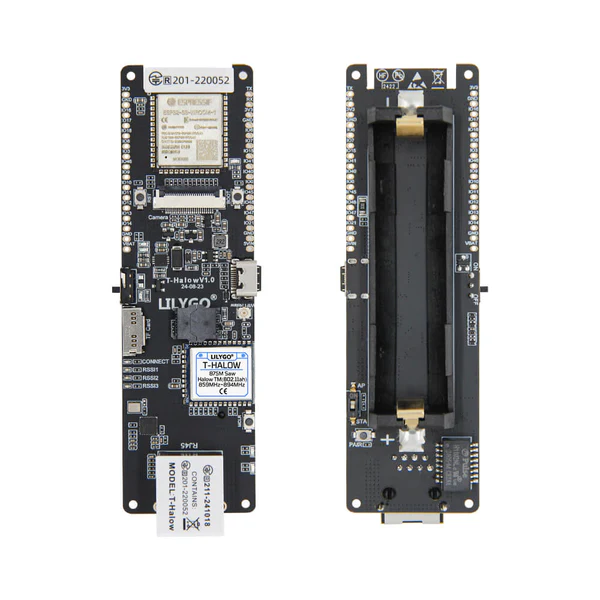
\includegraphics[width=1 \linewidth]{Documento/Imagenes/Análisis/Microcontroladores/lilygo-T-Halow.png}}
&
    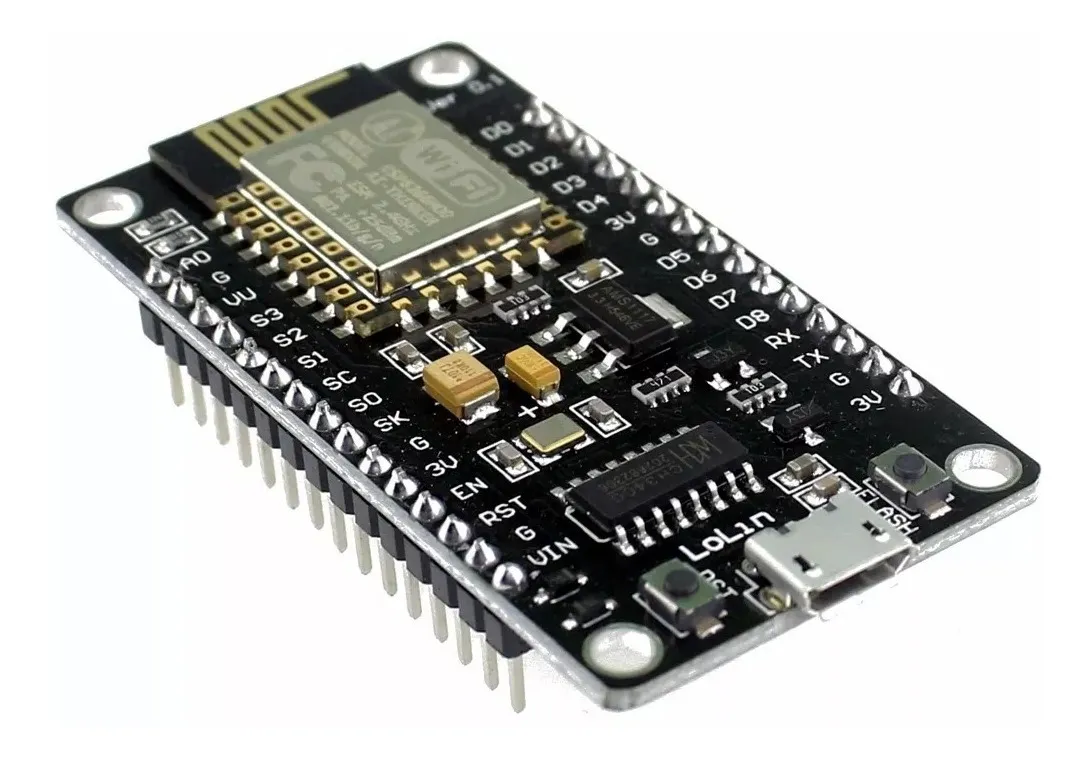
\includegraphics[width=1 \linewidth]{Documento/Imagenes/Análisis/Microcontroladores/NodeMCU.png}
&  
    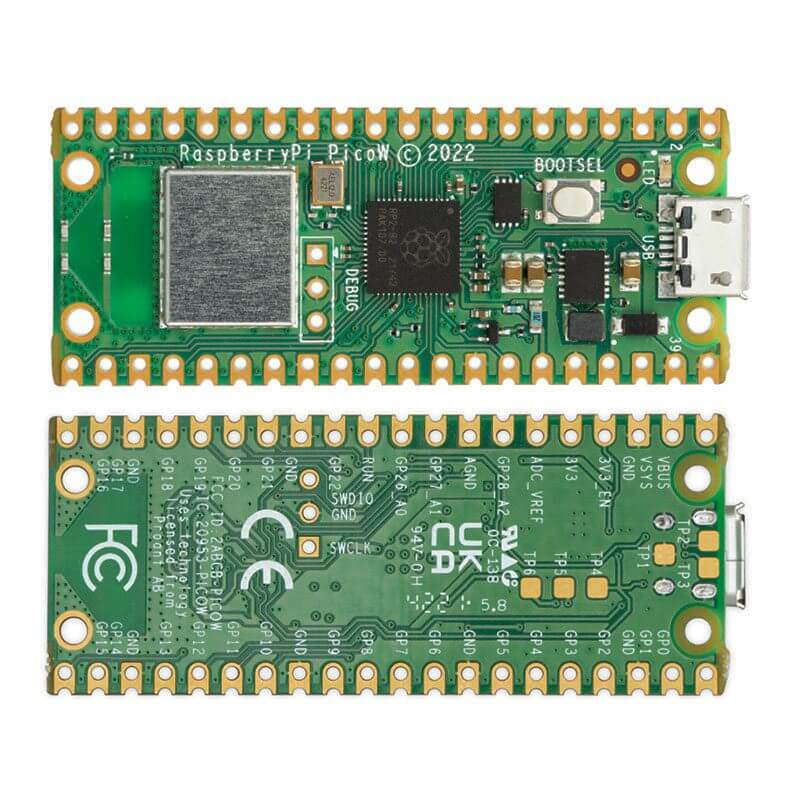
\includegraphics[width=0.9 \linewidth]{Documento/Imagenes/Análisis/Microcontroladores/RB Pico.jpg}   
\\ \hline

\end{longtable}




\begin{longtable}{|p{3cm}|p{4cm}|p{4cm}|p{4cm}|}
\hline
\multicolumn{4}{|c|}{Parte 2 Microcontroladores}\\
\hline
\textbf{Característica} 
& \textbf{Xiao ESP32-S3 R8} \cite{espressif2023_ESP32-S3}
& \textbf{STM32F103} \cite{stmicroelectronics2025_STM32F103ZE_datasheet}
& \textbf{ATmega328P} \cite{microchip2024_ATmega328P} \\
\hline
\endfirsthead

\hline
\textbf{Característica} 
& \textbf{Xiao ESP32-S3 R8} \cite{espressif2023_ESP32-S3}
& \textbf{STM32F103} \cite{stmicroelectronics2025_STM32F103ZE_datasheet}
& \textbf{ATmega328P} \cite{microchip2024_ATmega328P} \\
\hline
\endhead

\hline
\multicolumn{4}{r}{\textit{Continúa en la siguiente página}} \\
\endfoot

\hline
\endlastfoot

Arquitectura 
& Xtensa dual 32-bit LX7 
& ARM 32-bit M3 
& RISC 8-bit \\ \hline

Procesamiento 
& 240 MHz 
& 72 MHz 
& 16 MHz \\ \hline

RAM 
& 512KB + 8MB PSRAM 
& 64KB SRAM 
& 2KB SRAM \\ \hline

Flash 
& 8MB 
& 256–512KB 
& 32KB \\ \hline

Consumo Activo 
& 91 mA& 66 mA & 14 mA \\
Consumo Sleep & 240 \unit{\uA} & 8.5 mA & 60 \unit{\uA} \\ \hline

Voltaje & 3.3V & 5V & 5V \\ \hline

WiFi 
& 2.4GHz 
& No 
& No \\ \hline

Bluetooth 
& BLE 5 
& No 
& No \\ \hline

Sistema operativo (OS) 
& FreeRTOS 
& Bare-metal 
& Bare-metal \\ \hline

Costo (USD) 
& \$10–15 
& \$5 
& \$3 \\ \hline

Periféricos 
& \shortstack[l]{\\• 11 GPIOs\\• ADC (8 canales)\\• UART\\• SPI}
& \shortstack[l]{\\• 51 GPIOs\\• ADC (3 canales)\\• 5×UART\\• SPI}
& \shortstack[l]{\\• 23 GPIOs\\• ADC (8 canales)\\• USART\\• SPI} \\ \hline

Ventajas 
& \shortstack[l]{\\• RAM PSRAM (8MB)\\• Alto rendimiento\\• Bajo consumo \\• Compatible con \\tarjeta de expansión \\con cámara }
& \shortstack[l]{\\• Múltiples UARTs\\• Amplios GPIOs\\• Bajo costo}
& \shortstack[l]{\\• Amplia comunidad\\• Bajo consumo\\• Fácil prototipado} \\ \hline

Desventajas 
& \shortstack[l]{\\• GPIOs limitados\\• Costo moderado\\• Canales ADC\\ insuficientes}
& \shortstack[l]{\\• RAM limitada\\• Sin PSRAM\\• Procesamiento\\moderado}
& \shortstack[l]{\\• RAM mínima\\• Arquitectura 8-bit \\limitada} \\ \hline

Imagen 
& 
    \shortstack{\\ 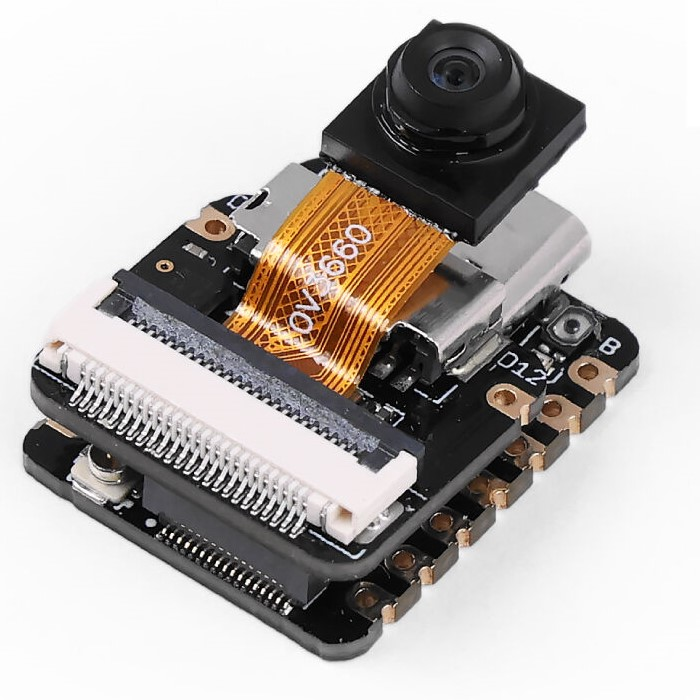
\includegraphics[width=1 \linewidth]{Documento/Imagenes/Análisis/Microcontroladores/xiao-esp32-s3-sense.jpg}}
&
    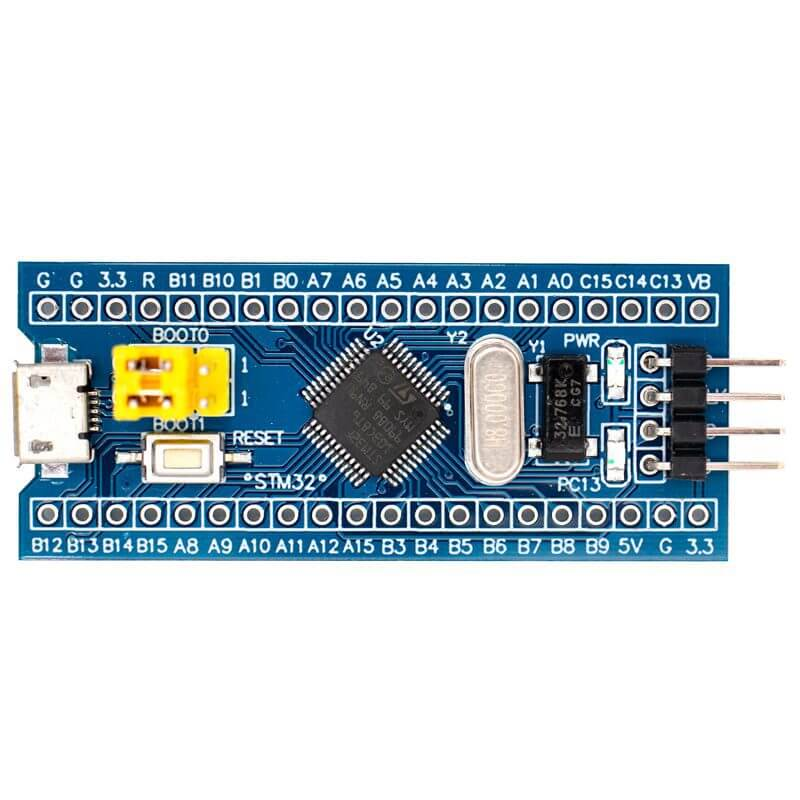
\includegraphics[width=1 \linewidth]{Documento/Imagenes/Análisis/Microcontroladores/STM32f103.jpg}
&  
    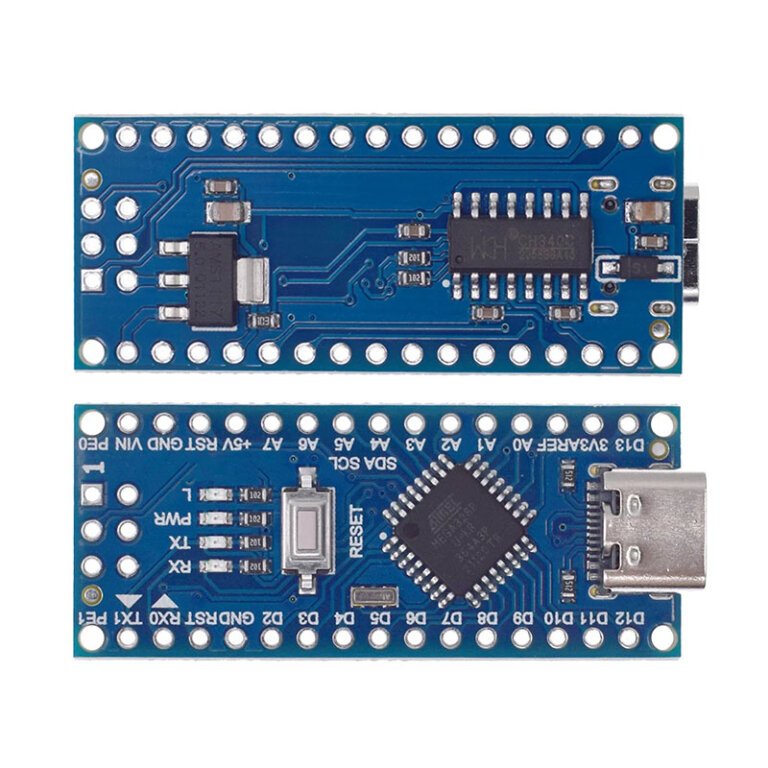
\includegraphics[width=0.9 \linewidth]{Documento/Imagenes/Análisis/Microcontroladores/Atmega328p.jpg}   
\\ \hline

\end{longtable}

\begin{longtable}{|p{3cm}|p{4cm}|p{4cm}|}
\hline
\multicolumn{3}{|c|}{Parte 3 Microcontroladores}\\
\hline
\textbf{Característica} 
& \textbf{Raspberry Pi Zero} \cite{raspberrypi_computers2025}
& \textbf{Raspberry Pi Zero 2 W} \cite{raspberrypi_computers2025}
 \\
\hline
\endfirsthead

\hline
\textbf{Característica} 
& \textbf{Raspberry Pi Zero} \cite{raspberrypi_computers2025}
& \textbf{Raspberry Pi Zero 2 W} \cite{raspberrypi_computers2025}
 \\
\hline
\endhead

\hline
\multicolumn{3}{r}{\textit{Continúa en la siguiente página}} \\
\endfoot

\hline
\endlastfoot

Arquitectura 
& ARM1176JZF-S 
& ARM Cortex-A53 (quad-core) 
 \\ \hline

Procesamiento 
& 1.0 GHz (single-core) 
& 1.0 GHz (quad-core) 
 \\ \hline

RAM 
& 512MB LPDDR2 
& 512MB LPDDR2 
 \\ \hline

Flash 
& microSD externa 
& microSD externa 
 \\ \hline

Consumo Activo 
&  2.5A
&  2.5A
 \\ \hline

Voltaje & 5V (microUSB) & 5V (microUSB)  \\ \hline

Broadcom chip & BCM2835 Single-core & RP3A0 Quad-core  \\ \hline

WiFi 
& Solo en modelo W: 2.4GHz (802.11n) 
& 2.4GHz (802.11n) 
 \\ \hline

Bluetooth 
& BLE 4.0 
& BLE 4.2 
 \\ \hline

Sistema operativo (OS) 
& Raspberry Pi OS (Linux) 
& Raspberry Pi OS (Linux) 
 \\ \hline

Costo (USD) 
& \$10 
& \$15 
 \\ \hline

Periféricos 
& \shortstack[l]{\\• 40 GPIOs\\• UART\\• SPI\\• I2C}
& \shortstack[l]{\\• 40 GPIOs\\• UART\\• SPI\\• I2C}
 \\ \hline

Ventajas 
& \shortstack[l]{\\• Bajo costo\\• Compatible con \\ecosistema Linux\\• Buena conectividad\\• Compacto}
& \shortstack[l]{\\• Multiprocesamiento \\(4 cores)\\• Más rápido que Zero\\• Ideal para visión\\ artificial}
 \\ \hline

Desventajas 
& \shortstack[l]{\\• Procesador antiguo\\• Capacidad de \\procesamiento limitada\\• Mayor consumo que \\MCUs}
& \shortstack[l]{\\• Sin GPIO analógicos\\• Requiere más energía \\que microcontroladores \\comunes}
 \\ \hline

Imagen 
& 
    \shortstack{\\ 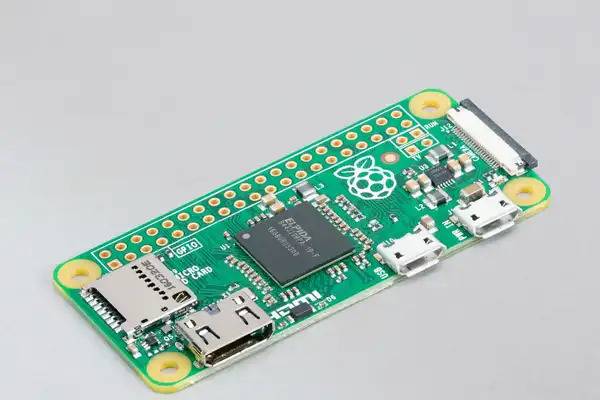
\includegraphics[width=0.9\linewidth]{Documento/Imagenes/Análisis/Microcontroladores/zerow.jpg}}
&
    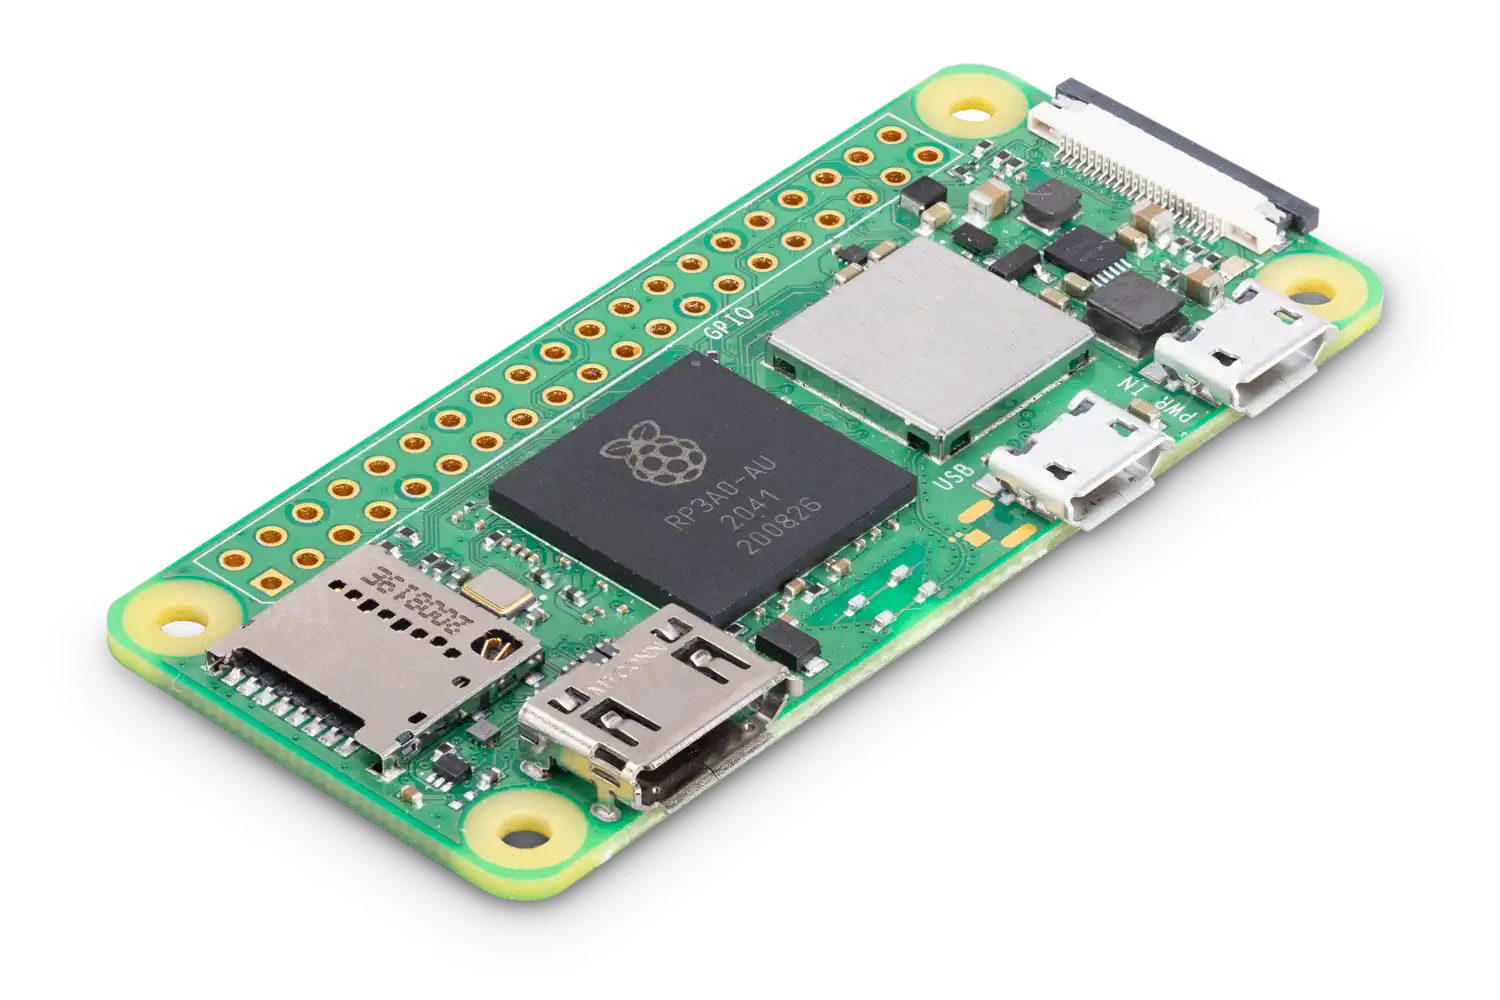
\includegraphics[width=0.9\linewidth]{Documento/Imagenes/Análisis/Microcontroladores/zero2w.jpg}

\\ \hline

\end{longtable}
